\chapter{Tabs-konceptet}
Udgangspunktet for beregningerne af en trådløs tjenestes fremkommelighed er en modellering af det effekt-tab, som radiosignalet har undervejs fra transmitteren til receiveren.
\section{ITU-R's koncept for tab over radio-forbindelser}
Et udbredt koncept ved anskuelse af transmissionstab er det, der allerede i 1951 første gang blev beskrevet af ITU i rekommendationen ITU-R P.341\cite{itur_p341-5}.

\begin{figure}[h]
	\centering
	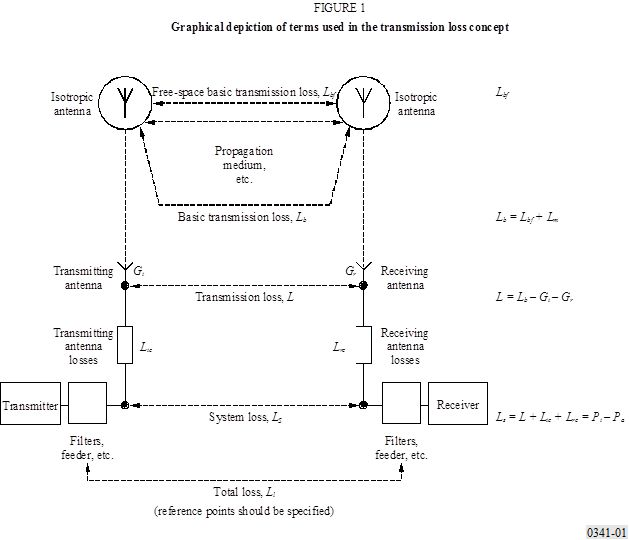
\includegraphics[width=0.8\textwidth]{figure/itur,P341-5,fig01.JPG}
	\caption{Rec. ITU.R P.341-5, figure 1, Graphical depiction of terms used in the transmission loss concept}
	\label{fig:zoner}
\end{figure}

Konceptet udmærker sig ved at isolere effekttab i radiokomponenter som antenner, filtre, bølgeledere, transceivere etc. fra effekttabet i radiosignalet på sin vej ind over landskabet.

Rekommendationen blev lavet i regnestokkenes tid, så alle effekter ($P$) er i $dB_m$ mens alle dæmpninger ($L$) og forstærkninger ($G$) er i $dB$.

\subsection{Systemtabet}
Det samlede tab i det viste koncept - kaldet ''\emph{systemtabet}'' - er det tab, signalet har fra transmitter til receiver, antennetab indbefattet. Modellen befatter sig ikke med tab i evt. filtre og bølgeledere. 

\begin{equation}
L_s =P_t -P_r
\end{equation}
hvor:
\begin{itemize}[]
 \item [$L_s$:] Tab for det samlede system
 \item [$P_t$:] Effekt afsendt af transmitteren (på udgangen af evt. filtre og bølgeledere) 
 \item [$P_r$:] Effekt modtaget af receiveren (på indgangen af evt. filtre og bølgeledere)
\end{itemize}

\subsection{Transmissionstabet}
\emph{Transmissionstabet ($L$)} er systemtabet uden tab i antennerne: 
\begin{equation}
L =L_s - L_{tx} - L_{rc}
\end{equation}
hvor:
\begin{itemize}[]
 \item [$L$:] Transmissionstabet
 \item [$L_s$:] Systemtabet 
 \item [$L_{tx}$:] Tab i senderantennen
 \item [$L_{rc}$:] Tab i modtageantennen
\end{itemize}

\subsection{Basistabet og antenneforstærkningen}
\emph{Basistabet ($L_b$)} er tabet over nogle teoretiske isotropiske (kugleformede) antenner, ækvivaleret med de faktiske antenner ved introduktionen af antenneforstærkningskonceptet: 
\begin{equation}
L_b =L + G_t + G_r
\end{equation}
hvor:
\begin{itemize}[]
	\item [$L_b$:] Basistabet 
	\item [$L$:] Transmissionstabet	
	\item [$G_t$:] Senderantennens forstærkning (i forhold til en isotrop antenne)
	\item [$G_r$:] Modtageantennens forstærkning (i forhold til en isotrop antenne)
\end{itemize}

Gevinsten ved indførelsen af antenneforstærkningskonceptet er, at man afkobler alle radiokomponenternes (incl. antennernes) karakteristika fra indflydelse på modellen for radiosignalets effekt-tab gennem luften over terrænet på sin vej fra sender til modtager. Definitionen på en antenne-forstærkning er givet i Annex 1, sektion 2 i ITU-R rekommendationen P.341\footnote{''The power gain of an antenna is defined as the ratio, usually expressed in decibels, of the power required at the input of a loss-free reference antenna to the power supplied to the input of the given antenna to produce, in a given direction, the same field strength or the same power flux-density at the same distance. When not specified otherwise, the gain refers to the direction of maximum radiation. The gain may be considered for a specified polarization.''} \cite{itur_p341-5}.

Sendendeeffekten ved den hypotetiske isotropiske sendeantenne er altså:
\begin{equation}
P_{it} = P_{t}+ G_t
\end{equation}
og modtageeffekten i den hypotetiske isotropiske modtageantenne bliver:
\begin{equation}
P_{ir} = P_{r}- G_r
\end{equation}
hvor:
\begin{itemize}[]
 \item [$P_{it}$:] Sendendeeffekten ud af den hypotetiske isotropiske sendeantenne 
 \item [$P_{t}$:] Sendendeeffekten ud af den faktiske sendeantenne
 \item [$P_{ir}$:] Modtageeeffekten ind i den hypotetiske isotropiske modtageantenne
 \item [$P_{r}$:] Modtageeeffekten ind i den faktiske modtageantenne
\end{itemize}
\FloatBarrier

\section{Longley-Rice's computer metode}
Et kendt eksempel på praktisk anvendelse af ITU's tabskoncept er den såkaldte Longley-Rice model. Denne model blev standard i U.S.A. allerede i 1965\cite{nbs-tn101}.

Longley og Rice havde kun 3 år efter - i 1968 - beskrevet en metode, hvorved man med en computer kan beregne tabet\cite{ntis-ad676874}.

Metoden dækker et stort dynamikområde. I tabel \ref{tab:lr-range} er området specificeret ud.

\begin{table}[h]
 \centering
 \begin{tabular}{ll}
   Parameter:                                   & Dynamikområde:\\
   \hline
   Frekvens                                     & 20 til 40.000 MHz\\
   Antennehøjde                                 & 0,5 til 3.000 m \\
   Distance                                     & 1 til 2.000 km \\
   Luftens brydningsindex (refraktivitet ($n$)) & 250 til 400 \\
 \end{tabular}
 \caption{Longley-Rice modellens dynamikområde}
 \label{tab:lr-range}
\end{table}
\FloatBarrier
\subsection{Den glatte kurve gennem terrænet}
Der laves en cirkelbue gennem terrænet mellem sende- og modtageantennen, således at cirkelbuen skærer gennem terrænnet under den laveste antennes mastefod. 

\subsubsection{Matematisk beskrivelse af terrænet ($\Delta h(d)$)}
Terrænets beskaffenhed tages ind i Longley-Rice modellen med blandt andet parameteren $\Delta h(d)$, som er middelværdien af højdeforskellene i terrænet mellem sende- og modtage-antennerne. Matematisk kan det skrives som:

\begin{equation}
\Delta h(d) = \sum\limits_{n=1}^N \frac{\Delta h_n}{\Delta d_n} \xrightarrow {N\rightarrow \infty} \Delta h
\end{equation}
hvor:
\begin{itemize}
	\item [$\Delta h_n = h_n - h_{n-1}$:] er terrænets højdetilvækst på positionen for den $n$'te måling [m]. 
	\item [$\Delta d_n = d_n - d_{n-1}$:] er afstanden mellem positionerne for den $n$'te og den $n-1$'te måling [km]. 
\end{itemize}


\subsubsection{Antennens effektive højde over terrænet}
Hvis terrænet var fladt, ville antennens effektive højde ($h_{e1,2}$) være lig med antennens strukturelle (faktiske) højde ($h_{g1,2}$) over terrænet.  
\begin{equation}
h_{e1,2} = h_{g1,2}
\end{equation}
hvor:
\begin{itemize}
	\item [$h_{e1,2}$:] er henholdsvis sende- og modtageantennens \emph{effektive} højde over jorden 
	\item [$h_{g1,2}$:] er henholdsvis sende- og modtageantennens \emph{faktiske} højde over jorden 
\end{itemize}

Hvis antennemasten står på terræn hævet over det omgivende terræn, ville antennens effektive højde ($h_{e1,2}$) være større med antennens strukturelle (faktiske) højde ($h_{g1,2}$) over terrænet.  
\begin{equation}
h_{e1,2} = h_{g1,2} + k \cdot exp(-2 \cdot \frac{h_{g1,2}}{\Delta h})
\end{equation}
hvor:
\begin{itemize}
	\item [$h_{e1,2}$:] er henholdsvis sende- og modtageantennens \emph{effektive} højde over jorden 
	\item [$h_{g1,2}$:] er henholdsvis sende- og modtageantennens \emph{faktiske} højde over jorden 
\end{itemize}
\FloatBarrier